\documentclass[twoside]{report}
\title{Seabass Style Sheet}
\author{Cephas Yeung}
\date{28/10/2024}
% MIT License

% Copyright (c) [2024] [Cephas Yeung]

% Permission is hereby granted, free of charge, to any person obtaining a copy
% of this software and associated documentation files (the "Software"), to deal
% in the Software without restriction, including without limitation the rights
% to use, copy, modify, merge, publish, distribute, sublicense, and/or sell
% copies of the Software, and to permit persons to whom the Software is
% furnished to do so, subject to the following conditions:

% The above copyright notice and this permission notice shall be included in all
% copies or substantial portions of the Software.

% THE SOFTWARE IS PROVIDED "AS IS", WITHOUT WARRANTY OF ANY KIND, EXPRESS OR
% IMPLIED, INCLUDING BUT NOT LIMITED TO THE WARRANTIES OF MERCHANTABILITY,
% FITNESS FOR A PARTICULAR PURPOSE AND NONINFRINGEMENT. IN NO EVENT SHALL THE
% AUTHORS OR COPYRIGHT HOLDERS BE LIABLE FOR ANY CLAIM, DAMAGES OR OTHER
% LIABILITY, WHETHER IN AN ACTION OF CONTRACT, TORT OR OTHERWISE, ARISING FROM,
% OUT OF OR IN CONNECTION WITH THE SOFTWARE OR THE USE OR OTHER DEALINGS IN THE
% SOFTWARE.
% 
% GitHub link:
% https://github.com/seabass6969/latex-template
\usepackage[utf8]{inputenc}

\usepackage{amsmath, amsfonts, amsthm, graphicx, geometry, lipsum}
\usepackage{hyperref}
\usepackage{minted}
\usepackage{blindtext, titlesec}
\makeatletter
\let\runauthor\@author
\let\runtitle\@title
\makeatother
\hypersetup {
    colorlinks=true,
    linkcolor=black,
    urlcolor=red,
    pdftitle={\runtitle}
}
\usepackage{verbatim, fancyvrb}

\usepackage{fancyhdr, lastpage}
\pagestyle{fancy}
\lhead{\runtitle}
\rhead{\runauthor}
\cfoot{Page \thepage \ of \pageref{LastPage}}
\usepackage{listings}


\patchcmd{\chapter}{\thispagestyle{plain}}{\thispagestyle{fancy}}{}{}
\expandafter\patchcmd\csname chapter*\endcsname{\thispagestyle{plain}}{\thispagestyle{fancy}}{}{}

\usepackage[Sonny]{fncychap}
\usepackage{xcolor-material}
\usepackage[svgnames]{xcolor}
\usepackage{tikz, tcolorbox}

\patchcmd{\thebibliography}{\chapter*}{\chapter}{}{}


\begin{document}
\maketitle
\tableofcontents

\chapter*{Introduction}
Introduction I am Cephas

\chapter{Useful packages}

\section{Hyperref}
My link to my \href{cephas.monster}{website}

\section{Verbatim}
\begin{Verbatim}[numbers=left, frame=single]
print("hello world")
\end{Verbatim}

\section{Colour}
I am {\color{red} red} and I am {\color{blue} blue}

\section{T colour box}

\begin{tcolorbox}[colback=red!5!white,colframe=red!75!black,title=My nice heading]
% \begin{lstlisting}[numbers=left, xleftmargin=5mm, language=python]
% print("hello world")
% \end{lstlisting}
test
\end{tcolorbox}
\section{Code}
\begin{minted}[bgcolor=Beige, linenos]{python3}
print("hello world")
test = "123"
for i in range(1,2):
    print(i)
\end{minted}

\section{Figures}
\begin{figure}[h]
    \centering
    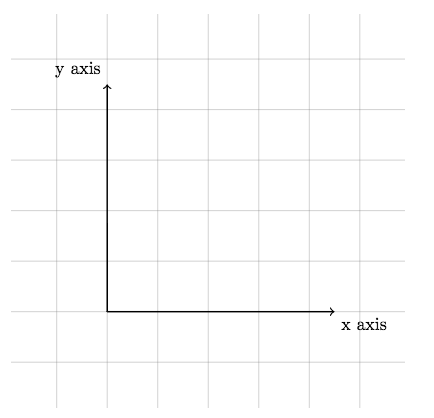
\includegraphics[scale=0.3]{image.png}
    \caption{I am a cartesian coordinate system}
    \label{fig:cartesian}
\end{figure}

\section{Bibliography}

I can reference Scipy \cite{2020SciPy-NMeth}

\section{Footnote}

I have a footnote here \footnote[1]{This is my footnote!}

\bibliographystyle{plain}
\bibliography{ref}

\end{document}